
%% In modeling fault-tolerant distributed systems, we want to be able to
%% address behavior and properties which depend on timing and communication
%% delay. For example, in the TTA startup protocol~\cite{Dutertre-Sorea-2004},
%% timing and transmission delays during synchronization are critical to
%% analyzing fault tolerance. 

%% Our language, \textbf{LIMA} addresses the three main
%% concerns implicit in this idea: fault modeling, specification of distributed
%% systems, and specification and analysis of systems with real-time constraints.

%We start by looking at the main syntactic elements of the language.
LIMA, which stands for ``\textbf{L}anguage for \textbf{I}ntegrated
\textbf{M}odeling and \textbf{A}nalysis'', is a domain specific
language embedded in the functional language Haskell~\cite{haskell98}. Its
implementation makes heavy use of Haskell as the host language for
expressing macros, enabling parametrization, and the handling of
parsing and low-level compilation.

The approach is an example of the embedded domain-specific language (EDSL) approach, which allows type-safe, Turing-complete compile time programming, and has been used in a number of domains, from embedded software~\cite{ivory-15} to runtime monitoring~\cite{pike-rv} to GPU programming~\cite{Chakravarty:2011:AHA:1926354.1926358}. Indeed, LIMA is built on the Atom EDSL~\cite{atom}. Atom was originally designed for bare metal embedded systems programming that supported concurrency without requiring a real-time operating system. The state machine language, in which the computation of individual nodes is expressed, is within the language of Atom~\footnote{Atom documentation can be found at \url{http://hackage.haskell.org/package/atom}.}.

We first present LIMA's syntax in Section~\ref{ssec:lima-syntax}. Then we describe code synthesis in LIMA in Section~\ref{ssec:code}. Formal model synthesis is presented in~\ref{ssec:formal-model-synth}. Finally, we briefly describe visualization tools associated with LIMA models in Section~\ref{ssec:lima-visualization}.

LIMA is designed to implement the desiderata described in Section~\ref{sec:towards-adsl}. However, as a initial implementation, some desiderata have not been fully implemented. We describe its current status below.

%%%%%%%%%%%%%%%%%%%%%%%%%%%%%%%%%%%%%%%%%%%%%%%%%%%%%%%%%%%%%%%%%%%%%%%%%%%%%%%%

\subsection{Syntax}\label{ssec:lima-syntax}


Our goal here is to introduce the LIMA. We are not, however, providing a comprehensive overview of the language, but we present the major elements. In particular, we elide the portion
of the language focused on building state machines internal to an
individual node or process. The node-local state machine language is described in the Atom itself.

We first introduce the basic building blocks of LIMA for modeling communicating state machines. Then we describe the LIMA fault model.

\subsubsection{Specifying Communicating State Machines}\label{sec:syntax}

There are
two main syntactic elements: \emph{atoms} and \emph{channels}.

\begin{itemize}
\item \emph{Channel}: Channels are typed and unidirectional. A channel is
declared in a monadic context as follows:
\begin{lima}
(tx, rx) <- channel name ini
\end{lima}
\noindent
creating two endpoints, \y{tx} and \y{rx}, that are user-defined
variables. These variables are ``handles'' for the channel that can be emitted
or read on, respectively. The types of \y{tx} and \y{rx} must agree in all
contexts. \y{name} is a plain text name for the channel, used to connect the
syntax at this level to the formal model and C code syntax after generation.
Finally, \y{ini} is an initial value for the contents of the channel.

% BFJ: include these or not?
%
% Channels also subsume the declaration of environmental signals. A clock tick
% and an interrupt signal are declared, respectively as follows:
% \begin{alltt}
% rx <- clock 5

% rx <- signal name (1`ms`)
% \end{alltt}
% \noindent

% The first declaration creates a clock that signals every 5 ticks,
% transmitted on a channel. The ``tick'' is a unit of time which is
% configurable in the backend.  Only a \y{rx} portion of the channel is
% created, since the clock is which creates the signal is outside of the
% model (and is created by the backend).  Likewise, a \y{signal} creates a
% named signal, together with a deadline for servicing the signal. The
% name denotes some external variable, such as a register.

\item \emph{Atom}: An atom defines a state machine that atomically
handles an incoming message, updates state, and possibly emits new
messages on other channels. An atom may, optionally, do this on a
specified period and phase.
%
\begin{lima}
myAtom rx tx = atom "myAtom" $ do
  v <- readChannel rx
  s <== value v
  writeChannel tx (Const 42)
\end{lima}
%
\noindent
The code above defines an atom named \y{``myAtom''} that handles
a message received on a channel with a receive handle \y{rx}. A channel
must be \emph{dereferenced} to extract a value from it. In the
declaration above, the dereferenced value, \y{v}, is stored into some
shared-state variable \y{s} whose scope exceeds the current definition,
and the value 42 is emitted on a channel with transmit handler \y{tx}. Here,
we use the term ``handler'' to mean a function that takes an incoming message
and returns an action to perform, usually doing some computation and sending
out new messages.

Atoms are hierarchical, i.e.\ an atom may contain other atoms and thus define a
hierarchy of global state variables and sub-atoms. All atoms declared
within a parent atom have access to the shared state of the parent. For example,

\begin{lima}
parent = atom "parent" $ do
  s <- int "sVar" 0
  atom "myAtom0" $ do
    ...
  atom "myAtom1" $ do
    ...
\end{lima}
\noindent
declares an atom named \y{``parent''} that contains a shared state
variable named \y{``s''} initialized to zero. It also contains two
handlers, \y{myAtom0} and \y{myAtom1}.
\end{itemize}

A typical pattern in the language is to declare a top-level atom as a
container for one or more channels and one or more sub-atoms which communicate
over the channels.

\begin{lima}
parent = atom "parent" $ do
  (tx, rx) <- channel "myChannel" 0
  s <- int "sVar" 0

  atom "myAtom0" $ do
    writeChannel tx 5

  atom "myAtom1" $ do
    cond $ fullChannel rx
    v <- readChannel rx
    s <== v
\end{lima}

\noindent
In this example, \y{myAtom0} sends the message \y{5} to \y{myAtom1} who stores
it directly in the shared variable \y{s}. The syntax \y{cond \$ \ldots}
declares a guard that must be true in order for the atomic action in that
block to be taken.

Finally, in addition to the hierarchical structure of shared state, the atom
to sub-atom relationship extends to guards. The execution of a sub-atom is
predicated not only on its guard condition, but also that of its parent, its
parent's parent, etc.

\subsubsection{Specifying Faults}

Here we  explain how we account for the fault models in LIMA, leaving the
technical details of how faults are encoded in the formal model to Section~\ref{ssec:fault-models}. Part of the philosophy behind our ADSL is that node
behavior and fault behavior should be separate in order to make reasoning
more modular. It is not a surprise then that the number and type of faults to
be included in the model is not specified along with the node behavior.
Instead, it is specified only in the compiler configuration.

Currently there are three options for fault model in LIMA:

\begin{itemize}
    \item \textbf{No Faults}. All nodes in the system perform as designed and channels
        deliver all messages on time.
    \item \textbf{Fixed Faults}. A mapping from node name to fault type is given,
        allowing the designer to specify statically the nature of faults to be
        considered.
    \item \textbf{Hybrid Fault Model}. The designer specifies numerical weights for
        each of three types of fault: manifest, symmetric, and byzantine. In
        this mode, the model-checker will explore all possible configurations
        of nodes with different faults as long as the weighted sum of
        node-fault combinations doesn't exceed a given total.
\end{itemize}
%
The last option is the most powerful form of reasoning about faults in the
system that LIMA offers. It generalizes the well-known results of Park and
Thambidari~\cite{Tha88:RDSS} and Lincoln and Rushby~\cite{Lincoln-Rushby}.

The fault model is decomposed from LIMA's atom's and channel model to specify communicating state machines. This is because we need to be able to synthesize executing code from the system; the fault model is used only within a formal verification. Thus, the fault model is presented as additional configuration data about the environment. The configuration is passed to the Sally model-checker compiler.


%%%%%%%%%%%%%%%%%%%%%%%%%%%%%%%%%%%%%%%%%%%%%%%%%%%%%%%%%%%%%%%%%%%%%%%%%%%%%%%%

%% \subsection{Backend Compilation Strategy}
%% \label{ssec:compilation-strategy}

\subsection{Code Synthesis}\label{ssec:code}

In the LIMA framework we can translate specifications into executable
implementations by generating C code. The code generator is optimized for
embedded targets, those running without a real-time operating system. Although,
the code also compiles and runs on POSIX systems as well.

At a high level, the code generator collects all the atomic actions given in
a specification and translates them into C functions which are executed on a
fixed, deterministic schedule. The schedule is determined by a scheduler which
takes into account each atom's preferred period and phase. The scheduler also
computes the number of basic expressions present in each atomic action so that
the real-time per tick can be calibrated. In section
\ref{ssec:formal-model-synth} we discuss synthesizing formal models from LIMA
specifications. By contrast, in the formal models the schedule is left
non-deterministic but fixed in each system trace.

\begin{figure}
\begin{lima}
ex4 :: Atom ()
ex4 = atom "ex4" $ do
  x <- int64 "x" 0
  y <- int64 "y" 0

  clocked 2 0 $ atom "atomX" $ do
    incr x
    decr y

  clocked 5 3 $ atom "atomY" $ do
    incr y

  assert "y not positive" (value y <=. 0)
\end{lima}
\caption{Example specification with two periodic atoms}
\label{fig:code-gen-example}
\end{figure}

As an example, consider the specification in Figure
\ref{fig:code-gen-example}. Two shared variables are declared and two periodic
atoms update their values. The code generator produces a C structure
representing the global system state; in this case it consists of two
integers. The fields of the struct are nested in several name spaces designed
to keep local variables in different atoms from conflicting. The two atomic
actions are translated into ``rules''; C functions that are called by a main
driver function. Figure \ref{fig:code-gen-rule} shows the rule generated for
\y{atomX}. Finally, the rule functions are driven by a scheduling function
that is responsible for maintaining a global clock value, executing the rules
in the correct order and time, and executing assertion statements. This is
shown in Figure \ref{fig:code-gen-scheduler}.

\begin{figure}
    \begin{lstlisting}[language=C,
                       numbers=left,
                       numberstyle=\scriptsize,
                       stepnumber=1,
                       numbersep=8pt,
                       showstringspaces=false,
                       breaklines=true,
                       frame=single]
struct {  /* state */
  struct {  /* ex4 */
    struct {  /* ex4 */
      int64_t x;
      int64_t y;
    } ex4;
  } ex4;
} state;
    \end{lstlisting}
    \caption{Global state structure in the generated C code}
    \label{fig:code-gen-state-struct}
\end{figure}


\begin{figure}
    \begin{lstlisting}[language=C,
                       numbers=left,
                       numberstyle=\scriptsize,
                       stepnumber=1,
                       numbersep=8pt,
                       showstringspaces=false,
                       breaklines=true,
                       frame=single]
/* Rule { 0, ex4.ex4.atomX } */
static void __r0() {
  bool __0 = true;
  int64_t __1 = state.ex4.ex4.x;
  int64_t __2 = 1LL;
  int64_t __3 = __1 + __2;
  int64_t __4 = state.ex4.ex4.y;
  int64_t __5 = __4 - __2;
  state.ex4.ex4.x = __3;
  state.ex4.ex4.y = __5;
}
    \end{lstlisting}
    \caption{Translated rule for \y{atomX}}
    \label{fig:code-gen-rule}
\end{figure}

\begin{figure}
    \begin{lstlisting}[language=C,
                       numbers=left,
                       numberstyle=\scriptsize,
                       stepnumber=1,
                       numbersep=8pt,
                       showstringspaces=false,
                       breaklines=true,
                       frame=single]
void ex4()
{
  {
    static uint8_t __scheduling_clock = 0;
    if (__scheduling_clock == 0) {
      __assertion_checks(); __r0();  /* Rule { 0, ex4.ex4.atomX } */
      __scheduling_clock = 1;
    }
    else {
      __scheduling_clock = __scheduling_clock - 1;
    }
  }
  {
    static uint8_t __scheduling_clock = 3;
    if (__scheduling_clock == 0) {
      __assertion_checks(); __r1();  /* Rule { 1, ex4.ex4.atomY } */
      __scheduling_clock = 4;
    }
    else {
      __scheduling_clock = __scheduling_clock - 1;
    }
  }
  __global_clock = __global_clock + 1;
}
    \end{lstlisting}
    \caption{Generated scheduler function}
    \label{fig:code-gen-scheduler}
\end{figure}

The final piece of C code generation is a user supplied \y{main} function
which should repeatedly call the generated scheduler function. This is
typically a tight loop with a call to the scheduler followed by a delay
statement that should be calibrated for the platform and desired amount of
real-time per system tick.

Auto-generated code like that shown in Figure \ref{fig:code-gen-scheduler} is only
meant to be machine readable, not human readable. One should think of this code as
an intermediate representation on the way to native machine code. It can be used
by human designers for debugging purposes if really needed, but the LIMA language and
complilation tool chain is setup to avoid exposing users to these low level details.

Execution of the generated code can be very useful in the design and debugging
of systems in LIMA. To that end LIMA provides several debugging features that
can be used along with forward execution in order to examine the state of the
system as it evolves over time. A special primitive function called \y{probe}
allows the user to setup a hook which monitors the value of any expression at
any point of a specification. These probes can be printed out as part of the
system execution by calling another special function \y{printProbe}. In Figure
\ref{fig:code-gen-probes}, the running example has been modified to include
probes on certain runtime expressions and to print the values of those
expressions out on every tick. The output generated during the example's
execution is shown in Figure \ref{fig:code-gen-print-probes}.

\begin{figure}
\begin{lima}
ex4 :: Atom ()
ex4 = atom "ex4" $ do
  x <- int64 "x" 0
  y <- int64 "y" 0

  clocked 2 0 $ atom "atomX" $ do
    incr x
    decr y
    probe "x + y" (value x + value y)

  clocked 5 3 $ atom "atomY" $ do
    incr y
    probe "y" (value y)

  assert "y not positive" (value y <=. 0)
  mapM_ printProbe =<< probes
\end{lima}
\caption{Probing the values of two runtime expressions}
\label{fig:code-gen-probes}
\end{figure}

\begin{figure}
\begin{plaintext}
y: -1
x + y: 0
y: -1
x + y: 0
y: -2
x + y: 0
y: -1
x + y: 1
y: -2
x + y: 1
y: -2
x + y: 1
y: -3
\end{plaintext}
\caption{Printing probes during execution}
\label{fig:code-gen-print-probes}
\end{figure}

% \begin{figure}
% \begin{lstlisting}[language=plaintext]
% Period  Phase  Exprs  Rule
% ------  -----  -----  ----
%      2      0      6  Rule { 0, ex4.ex4.atomX }
%      5      3      4  Rule { 1, ex4.ex4.atomY }
%                -----
%                   10
% \end{lstlisting}
% \caption{Scheduler output}
% \label{fig:code-gen-scheduler-output}
% \end{figure}


\subsection{Formal Model Synthesis}\label{ssec:formal-model-synth}

In this section, we describe our approach for mapping the syntax and semantics
of LIMA to a formal transition system model suitable for model checking.
(Translation to C code is relatively straightforward and we omit its
description here.) One of the main arrows of Figure~\ref{fig:overall_approach}
points from ADSL to ``formal models''.  In the following sections we describe
concretely how a system specified in LIMA can be translated into a
model-checker, while preserving important semantic constraints.

\emph{Efficiently} translating to a model-checking system without
relying on ad-hoc, problem-specific abstractions to make the translation
feasible is an open research problem that we focus on herein.

Let us return to our handler example from the previous section. Execution of
the handler updates the state of the system and so in our translation it is
represented by a transition relation. In Sally, transition relations are
specified by predicates over the ``current'' and ``next'' states of the
system. These are denoted by prefixing state variables with the namespaces
``state'' and ``next''.

\begin{figure}[ht]
\centering
\begin{lima}
handler rx tx = atom "someHandler" $ do
  let v = readChannel rx
  s <== v
  writeChannel tx (Const 42)
\end{lima}
\caption{Handler in the ADSL}
\label{fig:adsl-handler}
\end{figure}
%
%
\begin{figure}
\centering
\begin{sally}
;; someHndler:
(and msg_pending(state.cal, state.rx)
   (= next.s           msg_read(state.cal, state.rx))
   (= next.cal         msg_send(state.cal, state.tx, 42))
   (= next.other_var1  state.other_var1)
   (= next.other_var2  state.other_var2)
   ... )
\end{sally}
\caption{Handler as part of a formal model}
\label{fig:sally-handler}
\end{figure}

The variable \y{cal} in Figure~\ref{fig:sally-handler} is a state variable
referencing the ``calendar'', a data structure which keeps track of the times
that future events will take place. Sending a message is
implemented by adding a (future) time, channel identifier, and message content
to the calendar. At the proper time, a transition is enabled for the receiver
to act upon the message. This mechanism is described in more detail below. In
the Sally transition relation, the notations \texttt{msg\_pending(\ldots)},
\texttt{msg\_read(\ldots)}, and \texttt{msg\_send(\ldots)} are shorthand for more
complicated expressions:

\begin{itemize}
    \item \texttt{msg\_pending} is a boolean expression that checks whether
        there is a message available for delivery at the current time.
    \item \texttt{msg\_read} returns a message value from the appropriate
        entry in the calendar.
    \item \texttt{msg\_send(\ldots)} is an calendar-valued expression which
        computes the new value of the calendar, typically involving the
        overwrite of a calendar entry with the message contents and the overwrite
        of the entry's delivery time with the current time plus the configured
        message delay.
\end{itemize}

Various kinds of systems with real-time constraints can be implemented
on top of the calendar automata framework. In LIMA, two main
constructs are used to express features such as periodic execution
and aperiod timeouts. First, there is a primitive function \y{clocked},
which takes a concrete period value (in ticks) and either a concrete
phase value (between 0 and the period), or a special value that
indicates phase should be indeterminate. In this context, indeterminate
phase means that phase of execution is non-deterministic, but fixed
within each system trace. This allows us to explore phase-dependent properties
in real-time systems such as the Automatic Airbreak System case study presented in
\ref{airbuscs}.

Second, there is another primitive function \y{writeChannelWithDelay} which,
like \y{writeChannel}, sends a message over a channel, but with a specified
delay added to the delivery time. This feature can be used to program
reset-able, aperiodic timeouts. For example, in the following specification, a
node sets itself a timeout of 100 ticks, after which it sets a flag.

\begin{lima}
timeout = atom "timeout" $ do
  flag <- bool "flag" False
  (tx, rx) <- channel "self_loop" False
  writeChannelWithDelay 100 tx true

  atom "on_wake" $ do
    cond $ fullChannel rx
    flag <== true
\end{lima}

In this example, the relationship between the
outer atom and the inner atom is key. The \y{flag} and \y{channel} are shared between
the two atoms (being in scope for both of them), but the ``on\_wake'' atom's
execution is predicated on the guard of both itself, and its parent. Since
the parent has no guard in this case we can think of ``timeout'' and
``on\_wake'' as two different nodes communicating over the ``self\_loop''
channel.

% TODO: describe how faults are specified, but not how they are encoded, leaving
% that for later subsection.



%%%%%%%%%%%%%%%%%%%%%%%%%%%%%%%%%%%%%%%%%%%%%%%%%%%%%%%%%%%%%%%%%%%%%%%%%%%%%%%%

\subsubsection{Calendar Automata}\label{ssec:calendar}

Real-time system verification in general-purpose model-checkers
requires an explicit formalism of real-time progression. Trying to
encode real-time clocks directly is difficult; in particular, one
must avoid Zeno's paradox in which no progress is made because state
transitions simply update real-valued variables by an infinite
sequence of decreasing amounts whose sum is finite. To avoid this
problem, Dutetre and Sorea developed \emph{calendar
automata}~\cite{Dutertre-Sorea-2004}, which is itself inspired by
event calendars used in discrete-event simulation. Rather than
encoding ``how much time has passed since the last event'', it
encodes ``how far into the future is the next scheduled event'',
and a real-valued variable representing the current time is updated
to the next event time.

Define a set of \emph{events} $e_0, e_1, \ldots, e_n \in E$. For now, we
do not define events; intuitively, an event is a set of state variables
(shortly, we will associate events with messages sent in a distributed
system). When an event is \emph{enabled}, the transitions over events
are enabled; otherwise, the variables stutter (maintain the same value).

An \emph{event calendar} $\{ (e_0, t_0), (e_1, t_1), \ldots, (e_n, t_n)
\}$ is a set of ordered pairs $(e_i, t_i)$ called \emph{calendar events}
where $e_i \in E$ is an event and $t_i \in \mathbb{R}$ is a
\emph{timeout}, the time at which the event is scheduled. We denote
element $(e_i, t_i)$ of an event calendar by $c_i$.

Let $cal$ be an event calendar and $c_i, c_j \in cal$ be calendar
events. Define an ordering on calendar events such that $c_i \leq c_j$
iff $t_i \leq t_j$, and $\min(cal) = \{ c_i | \forall c_j \in cal, \,
c_i \leq c_j  \}$ are the minimum elements of $cal$.

Let a transition system $\mathcal{M} = (S, I, \rightarrow)$, be a set of
states $S$, a set of initial states $I \subseteq S$, and a transition
relation $\rightarrow \subseteq S \times S$. We implicitly assume a set
of state variables such that each state $\sigma \in S$ is a total
function that maps state variables to values. We sometimes prime a state
to denote that it satisfies the transition relation: $\sigma \rightarrow
\sigma'$. We also sometimes use a variable assignment notation to
describe what state variables are specifically updated: e.g., $\sigma' =
\sigma[v := v+1]$.

We distinguish two special state variables in a transition system: (1)
$now \in \mathbb{R}$ denotes the current time in the state, and (2)
$cal$ is an event calendar.

The following laws must hold of a transition system $\mathcal{M}$
implementing a calendar automaton:

\begin{enumerate}

\item \label{cal:a} Time is initialized to be less than or equal to
every calendar timeout: $\forall \sigma \in I$, $\forall (e_i, t_i) \in
\sigma(cal)$, $\sigma(now) \leq t_i$.

\item \label{cal:c} In all states, if the current time is strictly less
than every calendar event, then the only enabled transition is a
\emph{time progress} update: $\forall \sigma \in S$, $\forall (e_i, t_i)
\in \sigma(cal)$, if $\sigma(now) < t_i$, then $\forall \sigma'$ such
that $\sigma \rightarrow \sigma'$, $\sigma' = \sigma[now := \min(cal)]$.

\item \label{cal:d} In all states, if the current time equals a timeout,
then the only transitions enabled are calendar event updates associated
with the timeout: $\forall \sigma \in S$, $\exists (e_i, t_i) \in
\sigma(cal)$ such that $\sigma(now) = t_i$ implies $\forall \sigma'$
such that $\sigma \rightarrow \sigma'$, $\sigma'(now) = \sigma(now)$,
$\sigma'(c_j) = \sigma(c_j)$ for all $c_j \in \sigma(cal)$ such that
$c_j \neq c_i$ (recalling that by convention, $c_i = (e_i, t_i)$), and
$c_i \notin \sigma'(cal)$.

\end{enumerate}

From the definitions, it follows that in every state, the timeouts are
never in the past, and that time is monotonic:

\begin{lemma}[Future timeouts]\label{lem:ft} $\forall \sigma \in S$,
$(e_i, t_i) \in \sigma(cal)$, $\sigma(now) \leq t_i$.  \end{lemma}

\begin{lemma}[Monotonic time] $\forall \sigma, \sigma' \in S$, if
$\sigma \rightarrow \sigma'$, then $\sigma'(now) \geq \sigma(now)$.
\end{lemma}

Proofs of these two lemmas are straightforward and omitted.

In a distributed system, it is convenient to distinguish global actions
and local actions. Global actions are principally interprocess
communication, while local actions are those carried out by each process
to update its local state and produce new messages to broadcast. While
both global and local actions can both be modeled as events in a
calendar automata, doing so is generally overkill and complicates the
model. From the global perspective, individual processes can update
their local state atomically.

Again, following Dutetre and Sorea, we associate calendar events with
channels in a distributed system~\cite{Dutertre-Sorea-2004}. Specializing calendars to
message passing does not lose generality since all external
communication from an individual process can be abstracted as message
passing. Furthermore, fault models can be abstracted to act over
channels rather than processes~\cite{abstractions}. The calendar
introduces real-time constraints on when processes send and receive
messages.

Assume processes are indexed from a finite set $\Id$. A \emph{channel}
from process $i$ to $j$ is an ordered pair $(i,j)$. Fix a set of
messages $\Msg$. Given a channel and a timeout, let $send$ be a relation
on messages sent on a channel at a given time: $$send \subseteq \Id
\times \Id \times \mathbb{R} \times \Msg$$ So $send(i, j, t, m)$ holds
iff $i$ sends to $j$ message $m$ at time $t$. Likewise, let $$recv
\subseteq \Id \times \Id \times \mathbb{R} \times \Msg$$ be a relation
on messages received on a channel at a time, so that $recv(i, j, t, m)$
holds iff the message $m$ received by $j$ from $i$ at time $t$.

In the absence of faults, we require that messages received were
previously sent and not previously received: if $(i, j, t, m) \in recv$,
then $\exists t'$ such that $(i, j, t', m) \in recv$ where $t' < t$, and
$\neg\exists t''$ such that $t' < t'' < t$ and $(i, j, t'', m) = (i, j,
t, m)$. (We address faults in Section~\ref{ssec:fault-models}.)

Then an event calendar for sending and receiving messages on channels is
the union of the $send$ and $recv$ relations.

The event of receiving a message initiates a process to update its local
transition system and generate additional messages to send. When the
process is updating its local transition system, the event calendar is
paused. That is, updating an event $(i, j, t, m) \in recv$ also includes
updating $j$'s transition system.


%%%%%%%%%%%%%%%%%%%%%%%%%%%%%%%%%%%%%%%%%%%%%%%%%%%%%%%%%%%%%%%%%%%%%%%%%%%%%%%%

\subsubsection{System Properties}
\label{ssec:lima-properties}

In order to specify safety properties of a system in our ADSL, we've chosen to
use the synchronous observer pattern~\cite{Rushby-2012}. The synchronous
observer is a module that is composed with a target system synchronously. Its
job is to monitor the state variables of the system and raise a flag when
safety properties are violated. This idea is a popular alternative to
specifying properties in a special language (usually a temporal logic like
LTL) that has the advantage of being written in the same language and
environment as the system. Additionally, writing a synchronous observer is
second nature to the systems engineers; it is essentially like adding a runtime
check to a program.

Using observers allows us to sidestep the integration and expression of
temporal logic in our ADSL. Instead, the programmer adds an observer to her
system as a top-level monitor along with annotations that indicate which state
variables are to be observed.  From this we automatically generate a
corresponding observer module as well as the theorems and lemmas that the
model checker expects.

Our experiments with a few specific distributed fault-tolerant systems suggest
that using synchronous observers in place of LTL properties introduces very
little overhead during verification.


%%%%%%%%%%%%%%%%%%%%%%%%%%%%%%%%%%%%%%%%%%%%%%%%%%%%%%%%%%%%%%%%%%%%%%%%%%%%%%%%

\subsubsection{Fault Models}\label{ssec:fault-models}

The typical approach to modeling faults is to add new state variables to each process representing its fault state. Then a node chooses actions based on its fault state. As a simple example, we might define a node that sends a good message if it is non-faulty and a bad message otherwise. In pseudo-code using guarded commands, its definition might look like the following:

\small
\begin{verbatim}
node:
  health: Fault_Type;
  faulty(health)     --> send(bad_msg);
  non_faulty(health) --> send(good_msg);
\end{verbatim}
\normalsize

\noindent
But this approach mixes the specification of a node's behavior with
the fault model, an aspect of the environment. Generally, nodes do
not contain state variables assigned to their faults, or use their
fault-status to determine their behavior~\footnote{There are
exceptions; for example, benign faults may be detected by a node
itself (e.g., in a built-in-test).}! The upshot is that combining
faults and node state divorces the specification from its implementation.

A second difficulty with model-checking fault-tolerant systems in
general is that modeling faults requires adding state and
non-determinism. The minimum number of additional states that must
be introduced may depend non-obviously on other aspects of the fault
model, specific protocol, and system size. Such constraints lead
to ``meta-model'' reasoning, such as the following, in which Rushby
describes the number of data values that a particular protocol model
must include to model the full range of Byzantine faults (defined
later in this section):

\begin{quote} To achieve the full range of faulty behaviors, it
seems that a faulty source should be able to send a \emph{different}
incorrect value to each relay, and this requires $n$ different
values. It might seem that we need some additional incorrect values
so that faulty relays can exhibit their full range of behaviors.
It would certainly be safe to introduce additional values for this
purpose, but the performance of model checking is very sensitive
to the size of the state space, so there is a countervailing argument
against introducing additional values. A little thought will show
that $\ldots$. Hence, we decide against further extension to the
range of values~\cite{Rushby-OM1}. \end{quote}

The second problem is the most straightforward to solve. In
infinite-state model-checking, we can use either the integers or
the reals as the datatype for values. Fault-tolerant voting schemes,
such as a majority vote or mid-value selection (see Section~\ref{ssec:synchronous-om1}),
require only equality, or a total order, respectively, to be defined
for the data.

The solution to the first problem is more involved. Our solution
is to introduce what we call a \emph{synchronous kibitzer} that
symbolically injects faults into the model. The kibitzer decomposes
the state and transitions associated with the fault model from the
system itself. For the sake of concreteness in describing the
synchronous kibitzer, we focus on a particular fault model, the
hybrid fault model of Thambidurai and Park~\cite{Tha88:RDSS}. This fault
model distinguishes Byzantine, symmetric, and manifest faults. It
applies to broadcast systems in which a process is expected to
broadcast the same value to multiple receivers. A \emph{Byzantine}
(or \emph{arbitrary}) fault is one in which a process that is
intended to broadcast the same value to other processes may instead
broadcast arbitrary values to different receivers (including no
value or the correct value). A \emph{symmetric} fault is one in
which a process may broadcast the same, but incorrect, value to
other processes. Finally, a \emph{manifest} (or \emph{benign}) fault
is one in which a process's broadcast fault is detectable by the
receivers; e.g., by performing a cyclic redundancy check (CRC) or
because the value arrives outside of a predetermined window.

Define a set of fault types $$\textnormal{Faults} = \{none, byz,
sym, man\}.$$ As in the previous section, let $\Id$ be a finite set
of process indices, and let the variable $$faults: \Id \rightarrow
\textnormal{Faults}$$ range over possible mappings from processes
to faults.

The hybrid fault model assumes a broadcast model of communication.
Define $rnd: \mathbb{R} \rightarrow \mathbb{N}$ such that if
$rnd(t_0) < rnd(t_1)$, then $t_0 < t_1$.  A $broadcast: \Id \rightarrow
2^{\Id} \rightarrow \mathbb{R} \rightarrow \Msg \rightarrow 2^{E}$
takes a sender, a set of receivers, a real-time, and a message to
send each receiver, and returns a set of calendar events: $$broadcast(i,
R, t, m) = \{m | j \in R \textnormal{ and } send(i, j, t) = m\}$$

With this machinery, we can define the semantics of faults by
constraining the relationship between a message broadcast and the
values received by the recipients. For a nonfaulty process that
broadcasts, every recipient receives the sent message, and for
symmetric faults, there is no requirement that the messages sent
are the ones received, only that every recipient receives the same
value:

\noindent
\begin{center}
\begin{tabular}{l|l}
\begin{minipage}[t]{0.5\linewidth}
\[\begin{aligned}
&nonfaulty\_constraint =\\
  &\quad \forall i, j \in \Id, t \in \mathbb{R}.\\
  &\quad\quad\quad faults(i) = none\\
  &\quad\quad \textnormal{ implies } recv(i, j, t) = send(i, j, t)
\end{aligned}\]
\end{minipage}&
\begin{minipage}[t]{0.5\linewidth}
\[\begin{aligned}
&sym\_constraint =\\
  &\quad \forall i, j, k \in \Id, t \in \mathbb{R}.\\
  &\quad\quad\quad (\phantom{\textnormal{and }} faults(i) = sym\\
  &\quad\quad\quad \phantom{(}\textnormal{and } broadcast(i, \{j, k\}, t, m))\\
  &\quad\quad \textnormal{ implies } recv(i, j, t) = recv(i, k, t)
\end{aligned}\]
\end{minipage}
\end{tabular}
\end{center}

\noindent
Byzantine faults are left completely unconstrained.

Thus, faults can be modeled solely in terms of their effects on
sending and receiving messages. A node's specification does not
have to depend on its fault status directly.

Implementing the synchronous kibitzer fault injection in Sally
consists of three details. First, state variables are allocated for
each of the system nodes to represent its fault state. A state
variable is also allocated for each channel to represent potential
faulty values sent over that channel. These channel values are left
to vary non-deterministically through each system trace, but they
are constrained according the the fault type of the sender. For
example, if the sender is symmetrically faulty, then the fault
values of all its outgoing channels should be non-deterministic,
but equal. Second, these state variables are constrained by fault
model formulas generated by the compiler depending on the fault
model chosen in configuration.  In the general Hybrid Fault Model
case, these formulas are inequalities involving weighted sums over
the nodes. Last, the expression denoted by \y{msg\_read} in subsection
\ref{ssec:formal-model-synth} is a conditional. If the sending
node's fault state is non-faulty, then \y{msg\_read} returns the
intended message (a value that lives in some entry on the calendar).
If not, then \y{msg\_read} returns the (constrained) non-deterministic
fault value associated with the sender.

\subsection{Visualization}\label{ssec:lima-visualization}

We conclude this section by mentioning a third backend for LIMA that allows
system specifications to be visualized in various ways. To produce a
visualization one calls the \y{graphAtom} function with a filename prefix and
an \y{atom} specification. The result is a \y{png} image file containing an
abstract representation of the system. Nodes are displayed with their name in
diamonds. Atom/Subatom relationships are denoted with dotted black arrows and
channels are depicted by purple arrows. Figure \ref{fig:lima-visualization}
shows a typical example.

\begin{figure}
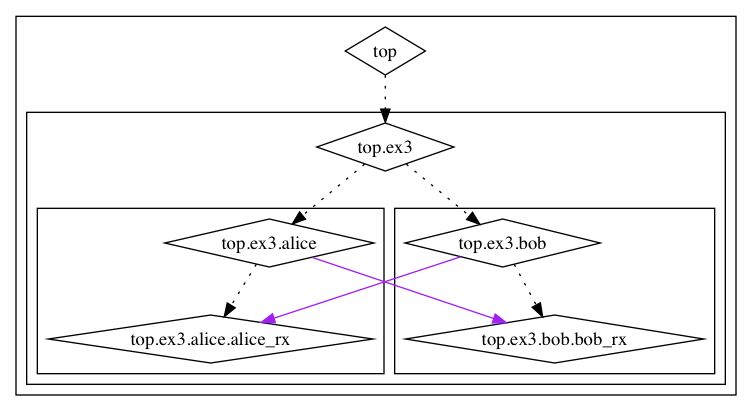
\includegraphics[scale=0.5]{periodic_ex3.png}
\caption{Graph representation of an atom specification}
\label{fig:lima-visualization}
\end{figure}

% If the $faults$ mapping is a constant, then faults are permanently
% but non-deterministically assigned to nodes. However, we can easily
% model \emph{transient faults} in which nodes are faulty temporarily
% by making $faults$ a state variable that is updated non-deterministically.
% Whether we model permanent or transient faults, a \emph{maximum
% fault assumption} (MFA) describes the maximum number of faults
% permitted in the system. The $faults$ mapping can be non-deterministically
% updated during execution while satisfying the MFA using a constraint
% such as $faults \in \{f \, | \, \mfa(f) \}$, where the MFA is defined
% by the function $\mfa$.


%%%%%%%%%%%%%%%%%%%%%%%%%%%%%%%%%%%%%%%%%%%%%%%%%%%%%%%%%%%%%%%%%%%%%%%%%%%%%%%%

%% BFJ: Other text, not used (yet?)

% BFJ: discussing clocks and signals seems lower priority than the semantics,
% especially since we haven't yet implemented them in LIMA.
%
% Finally, signals and clocks represent special types of channels whose transmit
% ends are thought of as being attached to external entities. The simplest way
% to model these parts of the system is to add them explicitly as modules. Clock
% and signal modules are responsible for setting timeouts, as in
% Figures~\ref{fig:node1-node2-modules} and \ref{fig:node1-node2-clock},
% and interecting with the calendar to effect the delivery of clock and signal
% messages to the correct nodes at the correct times.

% Calendar Automata are a useful and widely applicable modeling apparatus
% for real time systems which consist of discrete events. In this context,
% an \emph{event calendar} is a data structure consisting of a finite set
% of pairs $(e_i, t_i)$ where $e_i$ is an event which will occur
% (typically it contains the contents of a message), and $t_i \in
% \mathbb{R}$ is the time at which it will occur. A calendar process is
% added to the system which is in charge of updating the current time (a
% global). The process maintains the invariant that all items on the event
% calendar have times which are either equal to, or greater than, the
% current time. If there are events in the calendar tagged with the
% current time, transitions are enabled that carry out the event,
% including its removal. Only when all events are strictly in the future
% is the global time advanced to point of the next scheduled event.

% Channels of various kinds can be modeled using calendar automata. In this
% model, node A sends a message on a channel to node B by adding a future event
% to the calendar (at a time reflecting the transmission delay). Node B
% acts on the message once the global time is correct.

% The semantics of the ADSL described in Section~\ref{sec:adsl} map to this
% calendar framework and the necessary data structures and processes at the
% formal model level can be generated automatically.
